A poluição e uso irracional e inadequado da água comprometem a disponibilidade de água em padrões de qualidade apropriados 
ao uso da geração atual e das que estão por vir. Dessa maneira, faz-se necessário o monitoramento das águas que serão
destinadas ao abastecimento da população.

Os indicadores ambientais surgiram a partir da crescente preocupação socioambiental referente ao desenvolvimento.
Os indicadores tornaram-se fundamentais no processo decisório das políticas públicas e no acompanhamento de seus efeitos.
Esta dupla vertente apresenta-se como um desafio permanente de gerar indicadores e índices que tratem um número cada vez 
maior de informações, de forma sistemática e acessível, para os tomadores de decisão \cite{cetesbIndiceQualidadeH2O}.

Existe um indicador chamado Índice de Qualidade das Águas (IQA), o qual foi desenvolvido pela 
Companhia de Tecnologia de Saneamento Ambiental do Estado de São Paulo (CETESB) por meio da consulta à especialistas 
em qualidade da água, os quais apontaram parâmetros a serem avaliados acompanhados de seus respectivos pesos e a 
condição com que se apresenta cada parâmetro, de acordo com uma lista de valores. Desses parâmetros, os 9 (nove) 
principais foram selecionados. Para esses, foram estabelecidas curvas de variação de qualidade das águas de acordo 
com o estado ou a condição de cada parâmetro. Essas curvas são apresentadas na Figura ~\ref{graficos_parametros}.

A maior parte dos parâmetros levados em consideração no cálculo do IQA são indicadores de contaminação propiciada
pela emissão de esgotos domésticos.

O IQA é o principal índice de qualidade da água utilizado em todo o país. A finalidade de tal índice é transformar 
diversos dados relacionados à qualidade da água em um único número, que representa o nível de qualidade da água.

De acordo com a Agência Nacional de Águas \cite{anaGovIndicadores}, como desvantagens do uso do IQA, deve-se citar o fato de
o índice não contemplar vários parâmetros importantes para o abastecimento público, tais como:

\begin{itemize}
 \item Substâncias tóxicas (ex: metais pesados, pesticidas, compostos orgânicos);
 \item Protozoários patogênicos;
 \item Substâncias que interferem nas propriedades organolépticas da água.
\end{itemize}

Os nove parâmetros com seus respectivos pesos são apresentados a seguir:

\begin{figure}[!h]
\centering
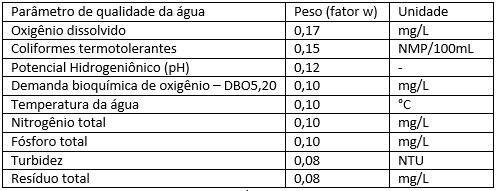
\includegraphics[scale=0.8]{editaveis/figuras/tabela_parametros_unidade}
\FloatBarrier
\label{tabela_parametros_unidade}
\caption[Parâmetros de qualidade da água do índice IQA e seus respectivos pesos]
  {Parâmetros de qualidade da água do índice IQA e seus respectivos pesos. \footnotemark}
\end{figure}
\footnotetext{Fonte: \cite{anaGovIndicadores}; \cite{cetesbIndiceQualidadeH2O}}

Além de seu peso ($w$), cada parâmetro possui um valor de qualidade ($q$), o qual é obtido do respectivo gráfico de qualidade
em função de sua concentração ou medida. Observe a figura abaixo:

\begin{figure}[!h]
\centering
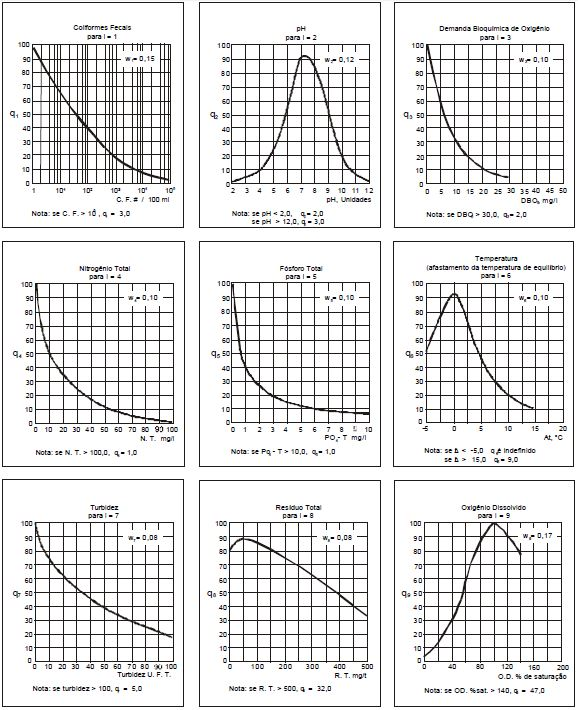
\includegraphics[scale=0.5]{editaveis/figuras/graficos_parametros}
\label{graficos_parametros}
\caption[Curvas de variação de qualidade das águas]{Curvas de variação de qualidade das águas.\footnotemark}
\end{figure}
\FloatBarrier
\footnotetext{Fonte: \cite{cetesbIndiceQualidadeH2O}}

O cálculo do IQA é dado da seguinte forma:

$$ IQA = \prod_{i = 0}^{n} {q_i}^{w_i} $$

\begin{center}
Fonte: \cite{anaGovIndicadores}
\end{center}

Onde:

\begin{itemize}
 \item $IQA$: Índice de Qualidade das Águas, representado por um número de 0 a 100;
 \item $q_i$: qualidade do i-ésimo parâmetro, representado por um número entre 0 e 100, obtido do respectivo gráfico de qualidade, em função de sua concentração ou medida;
 \item $w_i$: peso correspondente ao i-ésimo parâmetro fixado em função da sua importância para a conformação global da qualidade, isto é,  um número de 0 a 1, de forma que:
 
    $$ \sum_{i=1}^n w_i = 1 $$
    Sendo $n$ o número de parâmetros que entram no cálculo do IQA.
\end{itemize}

A tabela a seguir apresenta a classificação da água de acordo com o valor do IQA:

\begin{figure}[!h]
\centering
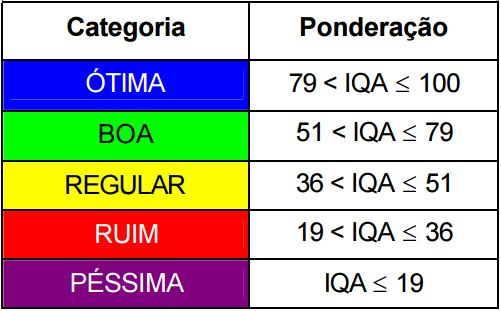
\includegraphics[scale=0.7]{editaveis/figuras/tabela_classificacao_IQA}
\label{tabela_classificacao_IQA}
\caption[Classificação da água de acordo com o IQA]{Classificação da água de acordo com o IQA.\footnotemark}
\end{figure}
\FloatBarrier
\footnotetext{Fonte: \cite{cetesbIndiceQualidadeH2O}}

Segundo a \cite{anaGovIndicadores}, a descrição dos parâmetros que compõe o IQA pode ser efetuada da seguinte maneira:

\begin{itemize}
 \item \textbf{Oxigênio dissolvido (OD)}: é um fator limitante para a manutenção da vida aquática e de processos de 
    autodepuração em sistemas aquáticos naturais e estações de tratamento de esgotos \cite{cetesbOxigenioDissolvido}.
    Águas limpas têm concentração de oxigênio, na maioria das vezes, maior ou igual a 5 mg/L. No que se refere aos processos que
    contribuem para a introdução do oxigênio na água, pode-se citar, além da fotossíntese, determinados processos físicos 
    os quais dependem das características hidráulicas dos corpos d’água, por exemplo: velocidade da água.
    
 \item \textbf{Coliformes termotolerantes}: São bactérias não patogênicas que ocorrem no trato intestinal de animais de sangue
    quente e são indicadoras de poluição da água causada pelos esgotos domésticos. Quando há grande quantidade dessas bactérias
    na água, há possibilidade de existir microorganismos capazes de transmitir doenças de veiculação hídrica.
    
 \item \textbf{Potencial Hidrogeniônico (pH)}: O pH (medida que determina a acidez ou basicidade de uma mistura) é capaz de
    alterar o metabolismo de diversas espécies aquáticas. Dessa forma, o CONAMA estabelece que o pH deve estar entre 6 e 9 
    para a proteção da vida aquática. O pH também afeta a intensidade do efeito das substâncias tóxicas nos seres aquáticos,
    tais quais os metais pesados.
    
 \item \textbf{Demanda Bioquímica de Oxigênio (DBO5,20)}: representa a quantidade necessária de oxigênio para oxidar a matéria
    orgânica aquática por meio da decomposição microbiana aeróbia. A ocorrência de altos valores de DBO5,20 acarreta na diminuição
    dos valores de oxigênio dissolvido (OD). A sigla DBO5,20 equivale à quantidade de oxigênio consumido em 5 dias a uma temperatura de 20C.
    A causa de altos valores de DBO5,20 numa amostra d’água é geralmente devido à emissão de dejetos de origem orgânica,
    principalmente esgotos domésticos.
    
 \item \textbf{Temperatura da água}: influencia em diversos parâmetros físico-químicos da água (ex: tensão superficial e a
    viscosidade) além de afetar o crescimento e reprodução de espécies aquáticas.
    
 \item \textbf{Nitrogênio total}: O nitrogênio pode ocorrer nos corpos d’água em diversas formas (orgânica, amoniacal, nitrito 
    e nitrato). Os nitratos são tóxicos aos humanos.
    Além disso, como os compostos de nitrogênio nutrem os processos biológicos, a grande concentração de nitrogênio 
    (juntamente com outros nutrientes) em corpos d’água causa a eutrofização, que prejudica o abastecimento público e
    a preservação da vida aquática.
    A principal fonte de nitrogênio em corpos d’água é o lançamento de esgotos sanitários e efluentes industriais.
    Em áreas agrícolas, o escoamento da água das chuvas em solos que receberam fertilizantes também é uma fonte de nitrogênio,
    assim como a drenagem de águas pluviais em áreas urbanas.
    
 \item \textbf{Fósforo total}: Assim como o nitrogênio, o fósforo (em excesso) causa a eutrofização das águas.
    As principais fontes de fósforo são os esgotos domésticos, pelo fato de eles terem a presença de detergentes
    superfostadados e das próprias fezes. Além disso, a drenagem pluvial de áreas agrícolas e urbanas também é uma fonte 
    significativa. Entre os efluentes industriais destacam-se os das indústrias de fertilizantes, alimentícias, laticínios, 
    frigoríficos e abatedouros.
    
 \item \textbf{Turbidez}: indica o grau de atenuação que um feixe de luz sofre ao atravessar a água. Tal atenuação é devida à
    absorção e espalhamento de luz causada pelos sólidos em suspensão. 
    A principal fonte de turbidez é a erosão dos solos (chuvas trazem os corpos sólidos).
    Porém, além desta, é possível citar as atividades de mineração, bem como o lançamento de esgotos e de efluentes industriais,
    como causadoras da turbidez nas águas.
    
 \item \textbf{Resíduo total}: é a matéria a qual permanece após a evaporação, secagem ou calcinação da amostra de água durante um 
    determinado tempo e temperatura.    
\end{itemize}

Existe uma empresa chamada Clean Environment Brasil \cite{cleanEnvironmentBrasil}, que fornece equipamentos de monitoramento e controle da água à ANA 
(Agência Nacional de Águas). Eles produzem várias sondas multiparamétricas (conseguem monitorar vários parâmetros em uma sósonda).

Seria interessante utilizar a sonda YSI EXO, que coleta dados de 6 sensores substituíveis, pois ela também é usada pela ANA para determinar a qualidade da água.

As opções de sensores para esse tipo de sonda são:

\begin{itemize}
 \item Oxigênio dissolvido;
 \item Matéria Orgânica Dissolvida (fluorescência);
 \item pH ou pH/ORP;
 \item Profundidade (que já é integrado);
 \item Algas totais (canal duplo para clorofila e algas azuis/verdes);
 \item Turbidez.
\end{itemize}

Assim, com apenas um equipamento relativamente leve (3,6 kg com baterias e sensores instalados) de pequenas
dimensões (phi = 7,62cm e comprimento = 71,10cm) é possível monitorar a maioria dos parâmetros do índice IQA \cite{cleanEnvironmentBrasil}.






